\subsection{Implementacija}
Zaradi simetrije problema bom delala v cilindričnih koordinatah. Za Laplaceov operator tako velja
\[ \nabla^2 u = \frac{1}{r} \pdv{}{r} \left( \frac{1}{r} \pdv{u}{r}\right)
+\pdv[2]{u}{z} =  \frac{1}{r} \pdv{u}{r} + \pdv[2]{u}{r} + \pdv[2]{u}{z},\]
oziroma diskretizirano:
\begin{align*}
    \pdv[2]{u(r,z)}{z} &= \frac{u_{i, j-1} - 2 u_{i,j} + u_{i,j+1}}{h^2}\\
    \pdv[2]{u(r,z)}{r} &= \frac{u_{i-1,j} - 2 u_{i,j} + u_{i+1,j}}{h^2}.
\end{align*}
Zaradi simetrije problema bi zadostovalo, da modeliramo samo pozitivne $r$, bi pa morali bržčas poskrbeti tudi za dodaten pogoj, da je pri $r=0$ toplotni tok v radialni smeri ničeln, zato sem raje modeliral cel interval $r \in [-1, 1 ]$.

Robne pogoje na plašču je lahko definirati: tam matrične elemente le postavimo na fiksni temperaturi. Na zgornji osnovni ploskvi je valj toplotno izoliran, zato tam toplotnega toka ne sme biti, kar je ekvivalentno pogoju, da je prvi odvod v navpični smeri ničeln. Analogno na spodnji osnovni ploskvi zahtevamo nek končen toploten tok, kar pomeni enak odvod v navpični smeri za vse matrične elemente pri $z=0.$

Obe podnalogi sem implementiral hkrati, saj je prva podnaloga le poseben primer druge. Zgornjo polovico sem držal na $T_1=-10$, spodnjo pa na $T_2 = 10$, za spodnjo osnovno ploskev sem predpisal toplotni tok v valj z vrednostjo 15.

Najprej sem pogledal Jacobijevo metodo z diskretizacijo na 10 točk v vsaki dimenziji. Uveril sem se, da metoda deluje tudi pri $r=0$ (ali bolje, da sem se točki pri $r=0$ uspešno izognil z izborom diskretizacije). Kot vidimo spodaj metoda tudi hitro konvergira.

\begin{center}
    \begin{minipage}{0.45\textwidth}
        \centering
    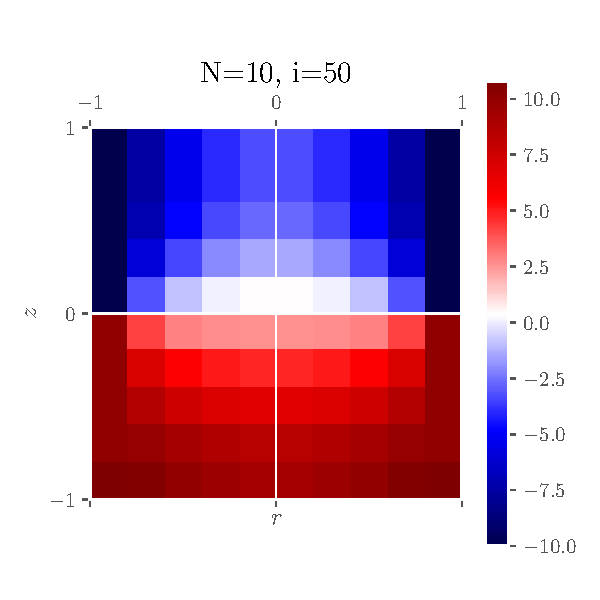
\includegraphics[width=\textwidth]{../old/2-valj-profili10_50.pdf}
    \caption{Temperaturno polje v prerezu valja po 50 korakih iteracije.}
    \end{minipage}\hfill
    \begin{minipage}{0.45\textwidth}
        \centering
    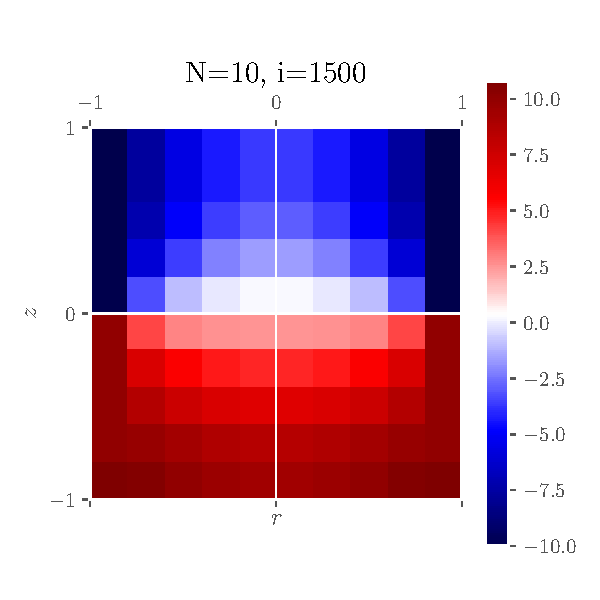
\includegraphics[width=\textwidth]{../old/2-valj-profili10_1500.pdf}
    \caption{Temperaturno polje v prerezu valja po 1500 korakih iteracije.}
    \end{minipage}
\end{center}

Nadaljeval sem s 50 točkami v vsaki dimenziji. Tu je sicer konvergenca počasnejša, se pa lepše opazijo atributi modela, predvsem pričakovano obnašanje pri zgornji osnovni ploskvi, kjer se izoterme sekajo s ploskvijo pod pravim kotom, kar pomeni pričakovano obnašanje, če naj tam ne bo toplotnega toka v ploskev.

\begin{center}
    \begin{minipage}{0.45\textwidth}
        \centering
    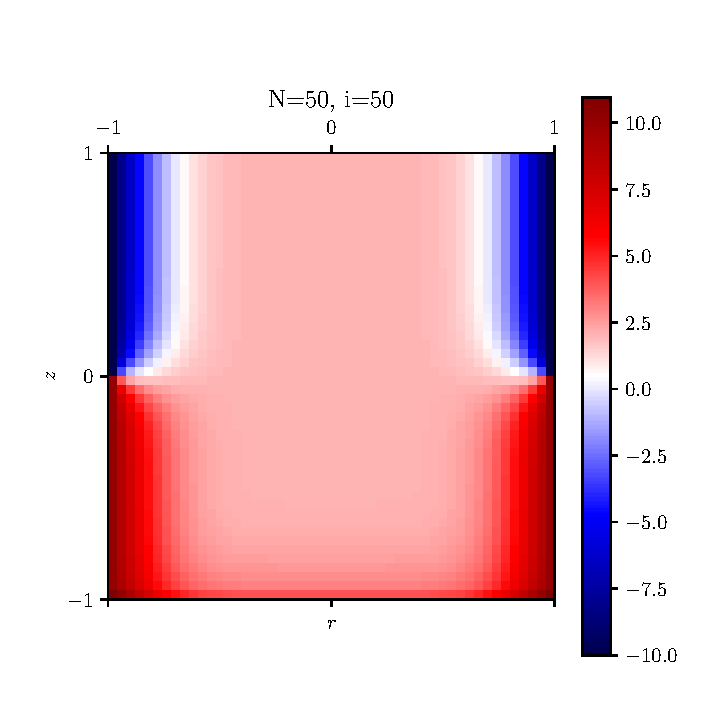
\includegraphics[width=\textwidth]{../old/2-valj-profili50_50.pdf}
    \caption{Temperaturno polje v prerezu valja po 50 korakih iteracije.}
    \end{minipage}\hfill
    \begin{minipage}{0.45\textwidth}
        \centering
    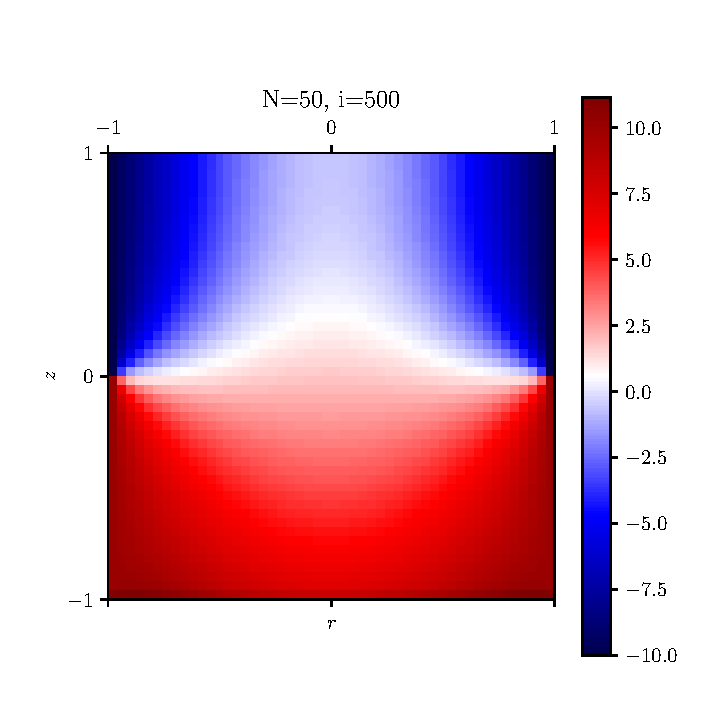
\includegraphics[width=\textwidth]{../old/2-valj-profili50_500.pdf}
    \caption{Temperaturno polje v prerezu valja po 500 korakih iteracije.}
    \end{minipage}

     \begin{minipage}{0.45\textwidth}
        \centering
    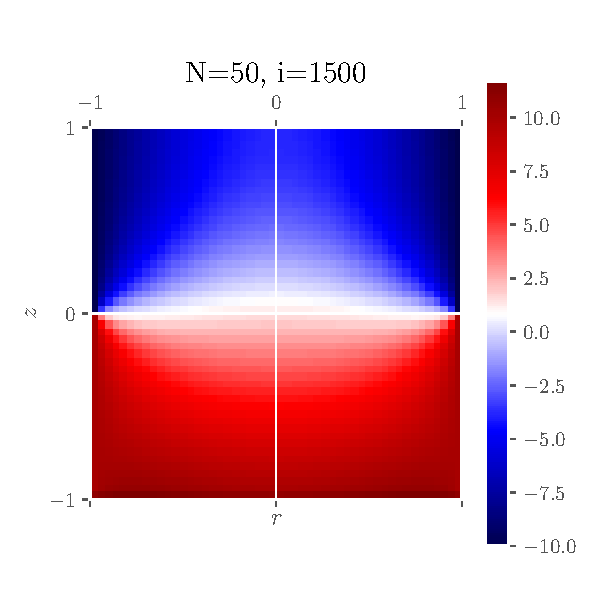
\includegraphics[width=\textwidth]{../old/2-valj-profili50_1500.pdf}
    \caption{Temperaturno polje v prerezu valja po 1500 korakih iteracije.}
    \end{minipage}\hfill
    \begin{minipage}{0.45\textwidth}
        \centering
    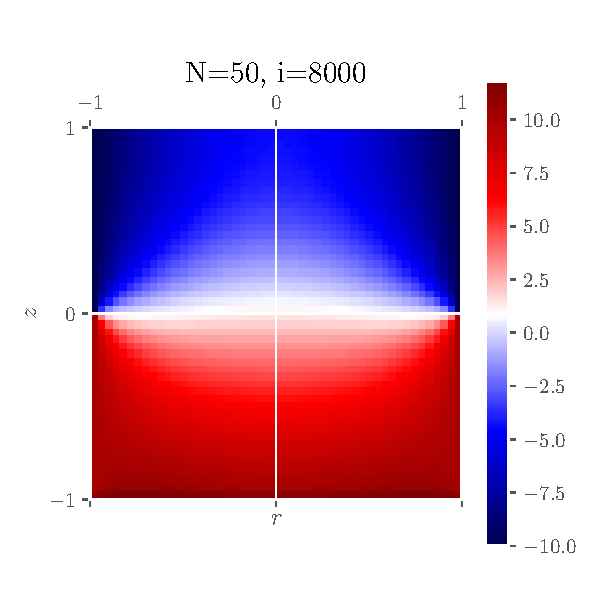
\includegraphics[width=\textwidth]{../old/2-valj-profili50_8000.pdf}
    \caption{Temperaturno polje v prerezu valja po 3000 korakih iteracije.}
    \end{minipage}
\end{center}

Nadaljeval sem s povečevanjem števila točk in opazovanjem konvergence. Kot je vidno na spodnjih slikah, pri 500 točkah v vsaki dimenziji tudi po 8000 iteracijah še ne dosežemo konvergence.

\begin{center}
    \begin{minipage}{0.45\textwidth}
        \centering
    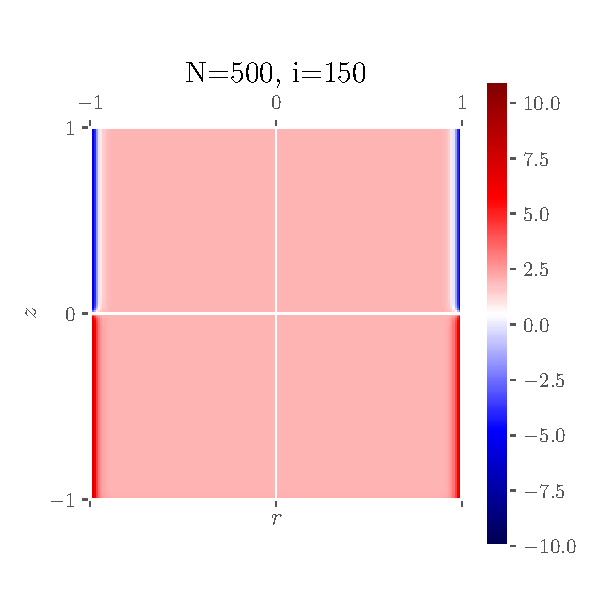
\includegraphics[width=\textwidth]{../old/2-valj-profili500_150.pdf}
    \caption{Temperaturno polje v prerezu valja po 50 korakih iteracije.}
    \end{minipage}\hfill
    \begin{minipage}{0.45\textwidth}
        \centering
    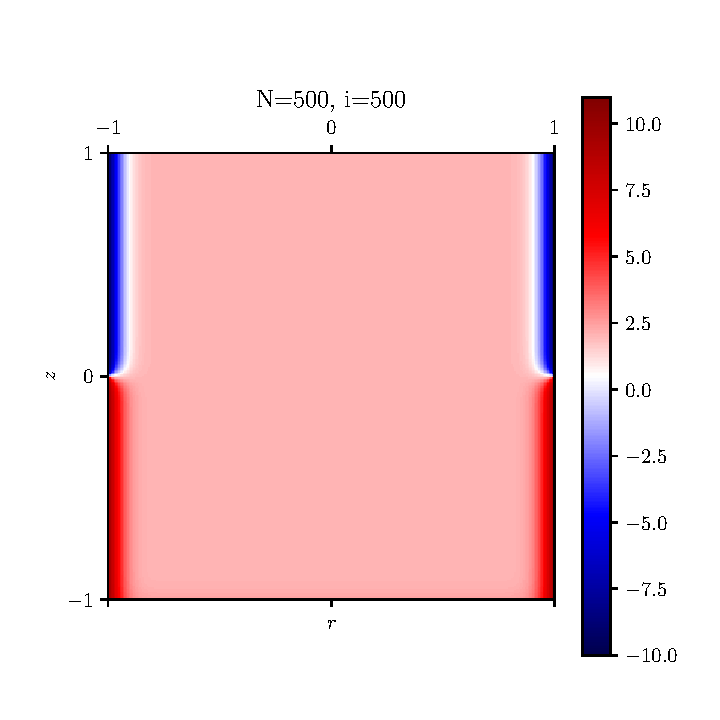
\includegraphics[width=\textwidth]{../old/2-valj-profili500_500.pdf}
    \caption{Temperaturno polje v prerezu valja po 500 korakih iteracije.}
    \end{minipage}

     \begin{minipage}{0.45\textwidth}
        \centering
    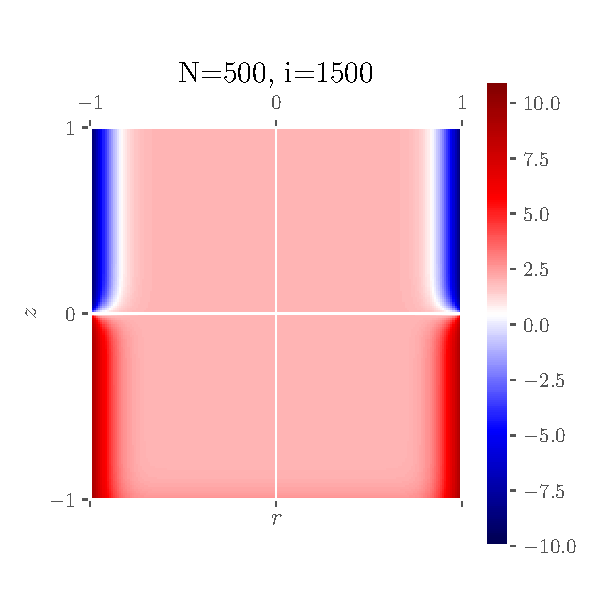
\includegraphics[width=\textwidth]{../old/2-valj-profili500_1500.pdf}
    \caption{Temperaturno polje v prerezu valja po 1500 korakih iteracije.}
    \end{minipage}\hfill
    \begin{minipage}{0.45\textwidth}
        \centering
    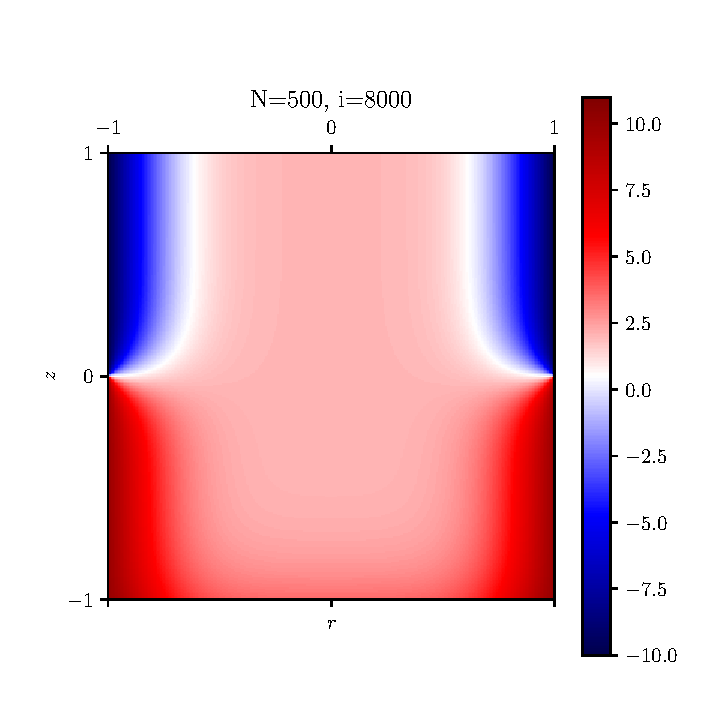
\includegraphics[width=\textwidth]{../old/2-valj-profili500_8000.pdf}
    \caption{Temperaturno polje v prerezu valja po 8000 korakih iteracije.}
    \end{minipage}
\end{center}
\subsection{Toplotna izolacija zgornje polovice valja}
Toplotno izolacijo modeliram tako, da zahtevam $\dpar{T}{r}=0$ na robu zgornje polovice plašča, kar dobim z izenačitvijo temperature drugega in predzadnjega elementa v vsaki vrstici s temperaturo prvega in zadnjega elementa. Kvalitativno se temperaturni profil ne spremeni drastično.
\begin{center}
    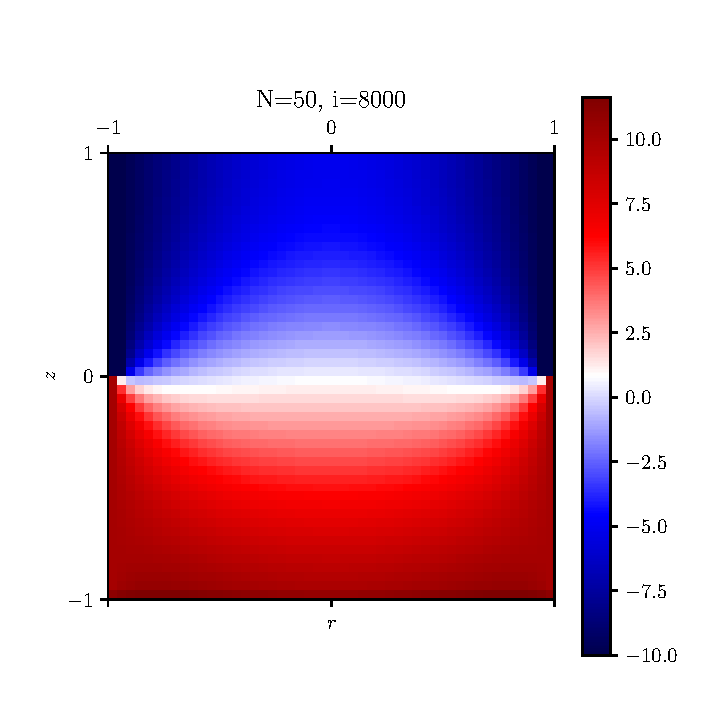
\includegraphics[width=0.5\textwidth]{../old/2-valj-profili50_8000_iso.pdf}
    \begin{minipage}{0.5\textwidth}
        Valj z izolirano zgornjo polovico plašča.
    \end{minipage}
\end{center}


\subsection{Pospešena relaksacija}

Pri vpeljavi pospešene iteracijske sheme sem imel tokrat več težav kot pri prejšnji nalogi. Iz neznanega razloga skaliranje parametra $\alpha$ s številom točk ni uspelo, kar je pomenilo več ugibanja in ročne optimizacije. Kot vidimo na sliki spodaj tudi rezultati niso bistveno pospešeni.
\begin{center}
    \begin{minipage}{0.45\textwidth}
        \centering
    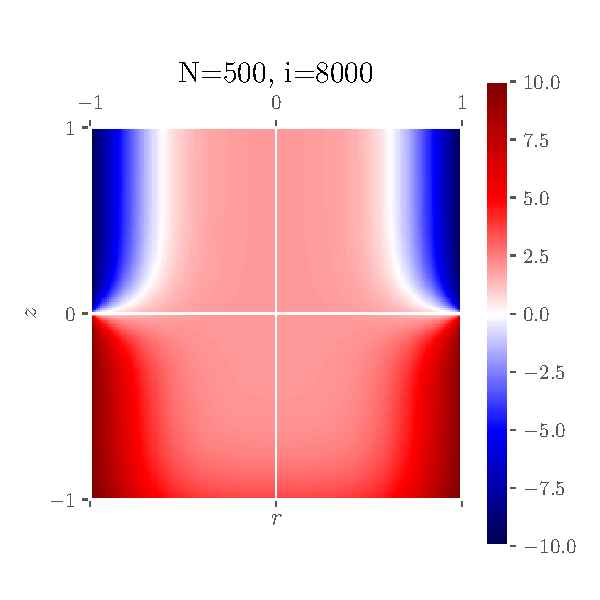
\includegraphics[width=\textwidth]{../old/2-valj-SOR.pdf}
    \caption{Končni rezultat po 8000 iteracijah mreže s 500 točkami. Stacionarnega stanja kljub pospešitvi nismo dosegli.}
    \end{minipage}\hfill
    \begin{minipage}{0.45\textwidth}
        \centering
        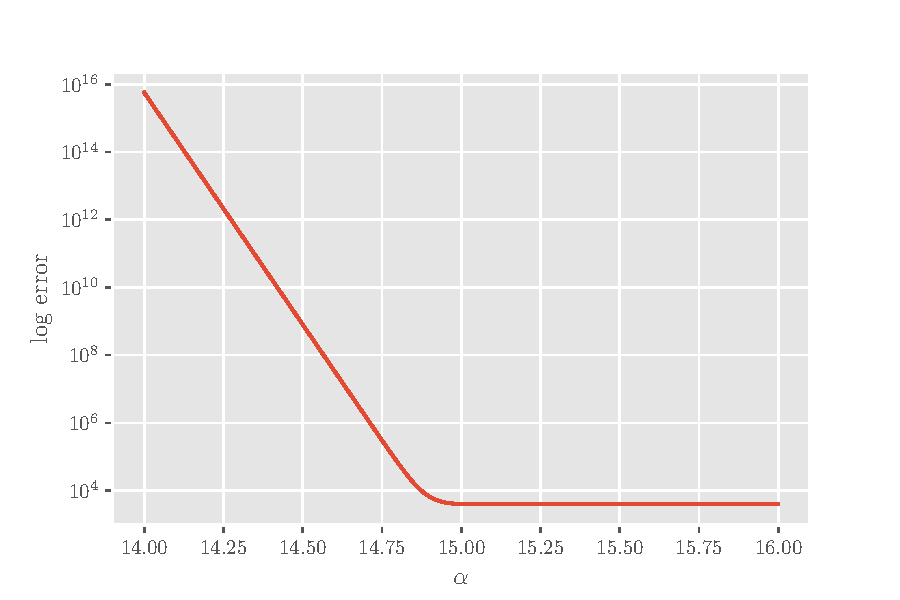
\includegraphics[width=1\textwidth]{../old/2-errors.pdf}
    \caption{Obnašanje pri iskanju optimalnega parametra $\alpha$.}
    \end{minipage}
\end{center}